\documentclass[preprint2]{aastex62}

\bibliographystyle{aasjournal}
\usepackage{graphicx}
\usepackage[suffix=]{epstopdf}
\usepackage{natbib}
\usepackage{amsmath}
\usepackage{url}
\usepackage{xspace}

%    Make Scientific Notation
\providecommand{\e}[1]{\ensuremath{\times 10^{#1}}}

% make the word Kepler italicized
\newcommand{\Kepler}{\textsl{Kepler}\xspace}



\begin{document}
%%%%%%%%%%%%%%%%%%%%%%
\title{Rotating Stars from \Kepler Observed with Gaia DR2}

\shorttitle{Rotating Stars from \Kepler Observed with Gaia DR2}
\shortauthors{Davenport et al.}


\correspondingauthor{James. R. A. Davenport}
\email{James.Davenport@wwu.edu}

\author{James. R. A. Davenport}
\altaffiliation{NSF Astronomy and Astrophysics Postdoctoral Fellow}
\altaffiliation{DIRAC Fellow}
\affiliation{Department of Physics \& Astronomy, Western Washington University, 516 High St., Bellingham, WA 98225, USA}
\affiliation{Department of Astronomy, University of Washington, Seattle, WA 98195, USA}


\author{Kevin R. Covey}
\affiliation{Department of Physics \& Astronomy, Western Washington University, 516 High St., Bellingham, WA 98225, USA}


 
 

%%%%%%%%%%%%%%%%%%%%%%%%%%%%%%
\begin{abstract}
We have matched the astrometric data from {\em Gaia} Data Release 2 to the sample of stars with measured rotation periods from \Kepler. Using 30,305 stars with good distance estimates, we select 16,248 as being likely main sequence single stars within a 0.5 mag region about a 1 Gyr isochrone. This removes sub-giants and unresolved binary stars from the sample.
The rotation period bimodality, originally discovered by \citet{mcquillan2013}, is recovered for stars out to 525pc, but is not detectable at further distances. 
We also find a significant width in the stellar main sequence of $M_G\sim$0.25 mag, as well as a  increase in the average rotation period correlated with the $M_G$ offset at a given color (mass). We interpret this to be the measurable change in luminosity and loss of angular momentum as stars evolve along the main sequence, which may provide a new independent test of stellar evolution and gyrochronlogy models.
This investigation represents the first step in understanding the star formation history of our solar neighborhood as traced through stellar angular momentum loss. 
\end{abstract}



%%%%%%%%%%%%%%%%%%%%%%%%%%%%%%
\section{Introduction}

The \Kepler mission \citep{borucki2010} a new era for enabling detailed study of angular momentum loss in low-mass stars. long noted as a means to possibly age-date stars (gyro), open clusters give hope that this general model works for low-mass stars
many Qs exist about details. these include Qs about initial rotation period distribution \citep[e.g.][]{barnes2010,matt2015}, the specific prescription for spin-down \citep{angus2015}, and exploring the efficiency of this angular momentum loss mechanism at old ages \citep{van-saders2016}.


one of the most compelling results from the rotation work in \Kepler is the discovery of a period bimodality. 
\citet{mcquillan2013} found bimodal feature, in M and later K stars \citep{mcquillan2014}. Davenport used Gaia DR1 to remove contamination from sub-giants and found the feature in G dwarfs. this feature proposed to be either a new short-lived transition or instability phase of momentum loss, or a signature of star formation history imprinted in the present-day rotation period distribution. However, to date this feature has only been observed in the \Kepler rotation period catalog, and most critically only for stars within $\sim$300 pc.



In this letter we follow the work of \citet{davenport2017} in studying the \Kepler rotation period sample using astrometric data from the {\em Gaia} mission \citep{gaia}. By matching the \citet{mcquillan2014} rotation period catalog to the newest data from {\em Gaia} Data Release 2 \citep{gaia_dr2}, we can use precise distances for essentially every star to select likely main sequence dwarfs to distances well over 1 kpc. Importantly this filters out both sub-giants (the main contaminant noted by \cite{davenport2017}), and unresolved binary stars.
Here we demonstrate the power of such a combined time-domain and astrometric sample for constraining the detailed evolution of main sequence stars themselves, and exploring the star formation history of the Milky Way.
 



%%%%%%%%%%%%%%%%%%%%%%
\section{The \Kepler--Gaia Data}

%Rotation periods in this study come from \citet{mcquillan2014}, who performed an Auto-Correlation Function analysis of \Kepler stars cooler than 6500 K that had at least $\sim$2 years of observation. The periods recovered from this approach generally agree very well with those found via Lomb-Scargle Periodograms \citep[e.g.][]{reinhold2013,aigrain2015}. Sources with multiple distinct periods, such as from binary systems with two spotted stars \citep[e.g.][]{lurie2015} are detected by \citet{mcquillan2014}, but are not included in the following analysis.

%The Gaia Data Release 1 (DR1) provides astrometric positions for over $10^9$ sources from the first year of observation with Gaia. The Tycho-Gaia Astrometric Solution (TGAS) measures improved proper motions and parallaxes for 2 million nearby, bright sources by extending the astrometric solutions from Tycho and Hipparcos. While the TGAS data are not a complete astrometric survey, and have possible systematics in the reported parallaxes \citep{gaia_dr1,stassun2016}, they represent a significant improvement in the astrometry and kinematics available for stars in the \Kepler field.


Our 
data xmatched by M. Bedell between \Kepler and Gaia DR2 (CITE). using 1arcsec radius, which included 195,830 sources with stellar properties from the \Kepler Data Release 25 and {\em Gaia} DR2.

sub-set was matched to the rotation catalog of \citet{mcquillan2014}

To select stars with good parallaxes, as well as high quality photometry from {\em Gaia}, we selected stars with the following criteria:
\begin{itemize}
\item Parallax error $< 0.1$ mas
\item $\sigma(M_{G}) / M_{G} < 0.01$
\item $\sigma(G_{BP}) /G_{BP} < 0.01$
\item $\sigma(G_{RP}) /G_{RP} < 0.01$
\end{itemize}

distances using the updated prescription from \citet{bailer-jones2018}
Following the suggested use of \citet{bailer-jones2018}, we use only sources with {\tt modality\_flag} == 1 (i.e. not a bimodal distance solution) and {\tt result\_flag} == 1 (i.e. well constrained distance).
              

Our final sample contained 30,305 stars in Gaia DR2 with measured \Kepler rotation periods that passed these selection criteria. A color--magnitude diagram of this sample is presented in Figure \ref{fig:cmd}, with points colored by their rotation periods.


\begin{figure}[]
\centering
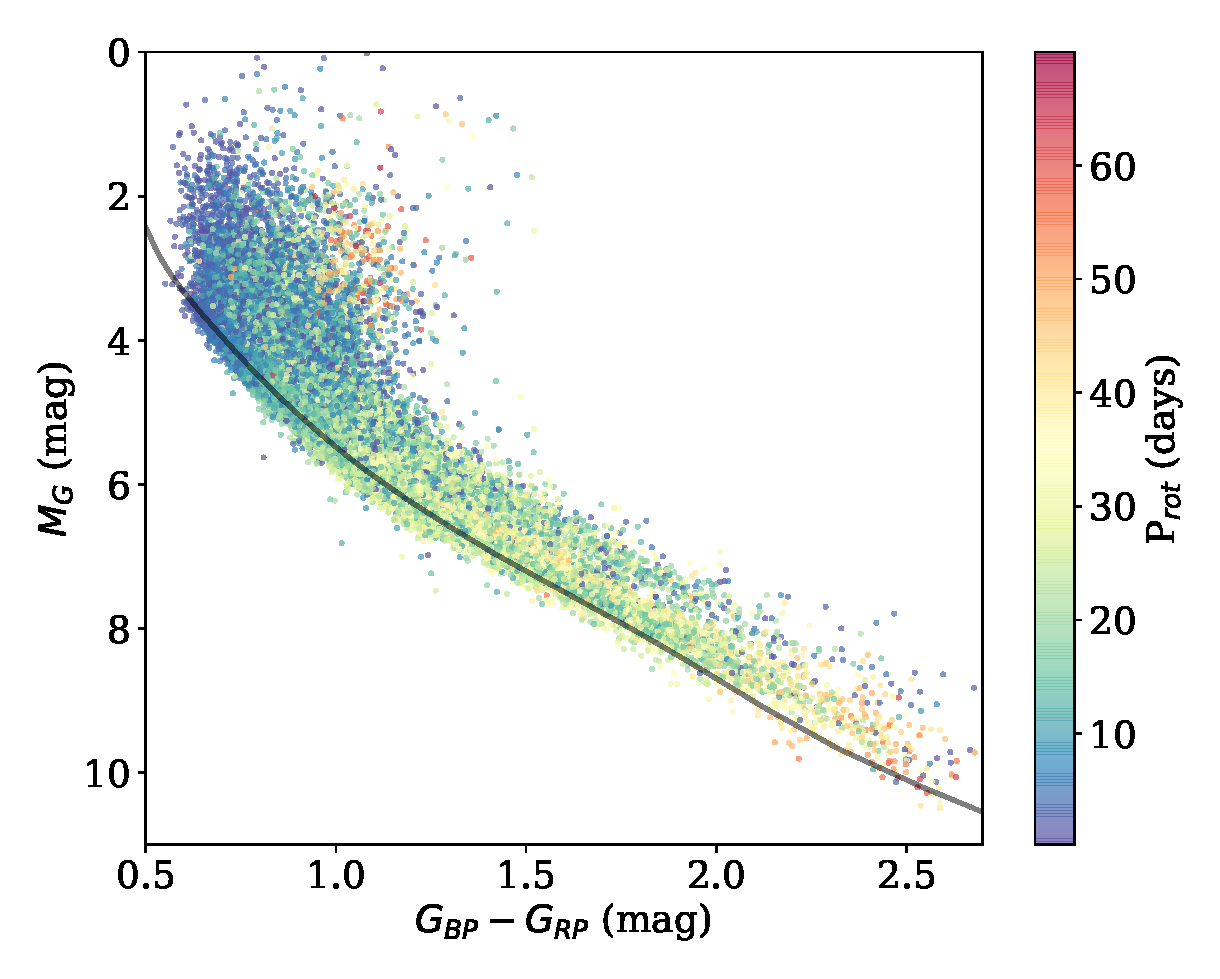
\includegraphics[width=3.6in]{../figures/cmd}
\caption{
Color--magnitude diagram for 30,305 \Kepler stars from the \citet{mcquillan2014} sample that are included in Gaia DR2, colored by their measured rotation period. For reference we show a $10^9$ year MIST isochrone (black line) used to select likely main sequence, single stars (black line). A track of binary  stars is apparent $\sim$0.75 mag above the main sequence. As in \citet{davenport2017}, we find significant contamination of the rotation period sample for bluer stars by sub-giants.}
\label{fig:cmd}
\end{figure}




%%%%%%%%%%%%%%%%%%%%%%
\section{Selecting Main Sequence Stars}

As in \citet{davenport2017}, the color--magnitude diagram shown in Figure \ref{fig:cmd} shows many of the bluer stars in the \citet{mcquillan2014} sample are significantly above the main sequence. These are likely subgiant stars, which do not follow the main sequence stars spin-down evolution \citep[e.g.][]{donascimento2012, van-saders2013}. Since \citet{davenport2017} found subgiants could obscure the rotation period bimodality for G dwarfs, these must be excluded from our analysis, but encourage future studies to explore the wealth of angular momentum evolution data from these most-main sequence objects.

Beyond the subgiant contamination above the main sequence, we can also see a secondary population of stars in a parallel track above the normal main sequence, which are likely unresolved binary stars. The pile-up above the main sequence occurs due to unresolved equal-mass field binaries, which was seen in the {\em Gaia} DR1 data as well \citep{anderson2017}. Since these systems may have experienced tidal evolution that could significantly impact their rotation evolution \citep[e.g.][]{lurie2017}, we must also remove these from our analysis. Though we do not explore the binary population in any detail here, this sample (perhaps with radial velocity follow-up) may provide useful insight into the tidal evolution of binary stars.

we use the Mesa Isochrones and Stellar Tracks \citep[MIST;][]{MIST} to describe the main sequence stars in Figure \ref{fig:cmd} using [Fe/H] =0.25, and an age of $10^9$ years.
main seq stars chosen in 0.5 mag window





%Though \citet{mcquillan2014} attempted to only measure periods for dwarf stars, the sample of \Kepler--Gaia matched stars contains both main sequence dwarfs and evolved stars (giants and subgiants). Previous studies have shown  significant contamination by giants or subgiants can affect the implied variability properties of dwarf stars \citep{ciardi2011,mann2012}. Therefore to properly understand the nature of the period distribution and its implications for age-dating field stars, a robust sample of main sequence stars must be selected.
%
%Faint stars were removed by requiring sources have $G$-band flux errors $<1$\%. To ensure accurate distances, and therefore luminosities, parallaxes were required to have errors $<0.4$ mas. These cuts left a total of 894 stars from the \Kepler--TGAS matched sample (68\%). The Hertzsprung--Russell (HR) diagram for these stars is shown in Figure \ref{fig:HR}, with each point colored by its \Kepler-measured rotation period. Example isochrones from the \citet{bressan2012} grid are shown for two ages. A systematic offset of $\sim$0.5 magnitudes is found between the measured absolute $G$-band and the isochrone's main sequence. This offset is likely due to calibration differences between the nominal and actual $G$-band (A. Brown, private communication).
%
%
%The HR-period diagram in Figure \ref{fig:HR} shows stars with a range of evolutionary states, and could help test post-main sequence angular momentum evolution models \citep[e.g.][]{donascimento2012}. Outliers in this diagram are either due to erroneous cross-matching in the \Kepler and Gaia catalogs, or represent interesting systems such as rare binary star configurations or stars that have undergone mergers or ingested giant planets \citep{massarotti2008,tayar2015}. For example, examining the 2 Micron All Sky Survey \citep[2MASS][]{2mass} image on SIMBAD for 
%the rapidly rotating star at $T_{eff}=4500$ K, $M_G=4.5$ mag, $P_{rot}$=0.652 d, in Figure \ref{fig:HR} (KIC 07957709), this source appears highly contaminated with three point sources clustered within $\sim$10 arcseconds, likely leading to an erroneous position in the HR diagram, and possibly incorrect variability measurements with \Kepler.
%Investigating all such outliers in Figure \ref{fig:HR} is beyond the scope of this work, but these targets are worth further study as they may reveal new physics.
%
%
%
%Main sequence stars were selected using a simple cut around 300 Myr isochrone. Given the systematic offset of $\sim$0.5 mag between the Myr isochrone and the observed $M_G$ values, a fairly wide band of stars ($0\le \Delta M_G \le 1$) was selected as being ``close to the main sequence''. The final sample included 440 stars. This simplistic cut is not a robust dwarf--giant, nor single--binary star separator, but serves to select a sample of mostly main sequence stars for the illustrative purpose of this work. More precise selection will require an improved isochrone track, as well as updated parallaxes from the full Gaia DR2.
%



%%%%%%%%%%%%%%%%%%%%%%%
%\section{Extending the Spin-Down Gap}
%A bimodal period distribution was first discovered by \citet{mcquillan2013} for \Kepler M dwarfs, who found a dearth of objects with periods around $\sim$25 days. Follow-up work by \citet{mcquillan2014} found this bimodality extended to K dwarfs, up to $T_{eff}\sim5500$. Figure \ref{fig:gyro} shows the rotation period distribution for the final 440 star sample of likely main sequence stars. The bimodality appears to extend smoothly through to the hottest stars in this sample. 
%
%While these periods for field stars were robustly measured by \citet{mcquillan2014} and others, the bimodality did not appear in previous \Kepler work due to the high contamination rate by subgiants for these bluer, hotter stars.  414 rotating stars had acceptable photometric and parallax uncertainties in TGAS, but were culled from this sample for having $M_G$ luminosities higher than the main sequence cut in \S3 above. Note that distributions of $\log g$ values from the Kepler Input Catalog \citep{brown2011a} for both the main sequence and subgiant stars were not statistically different.






\begin{figure*}[]
\centering
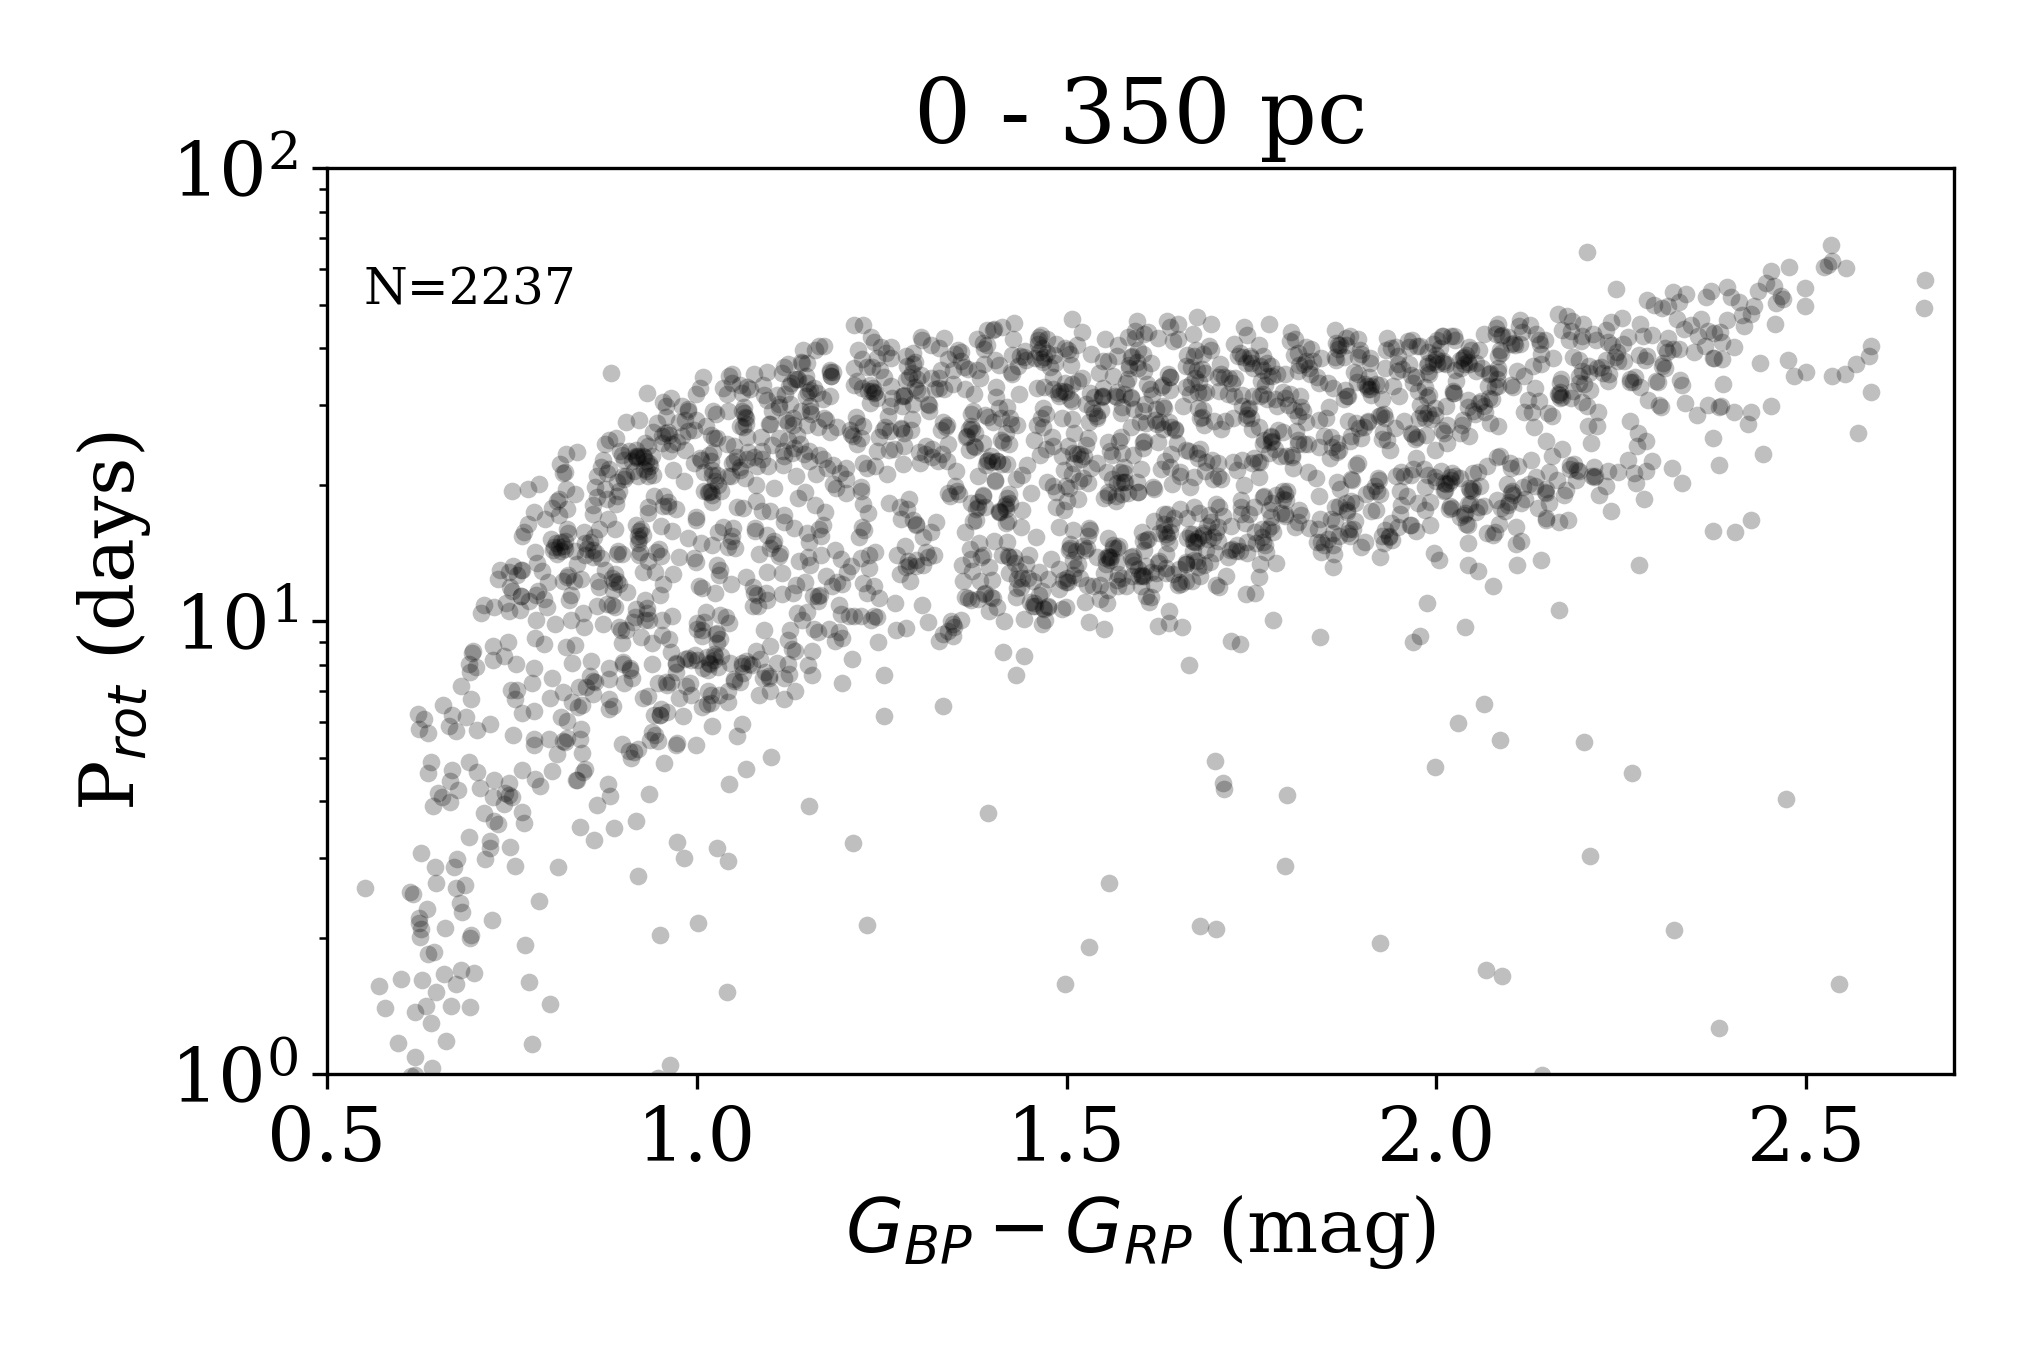
\includegraphics[width=3.5in]{../figures/rot_dist_0}
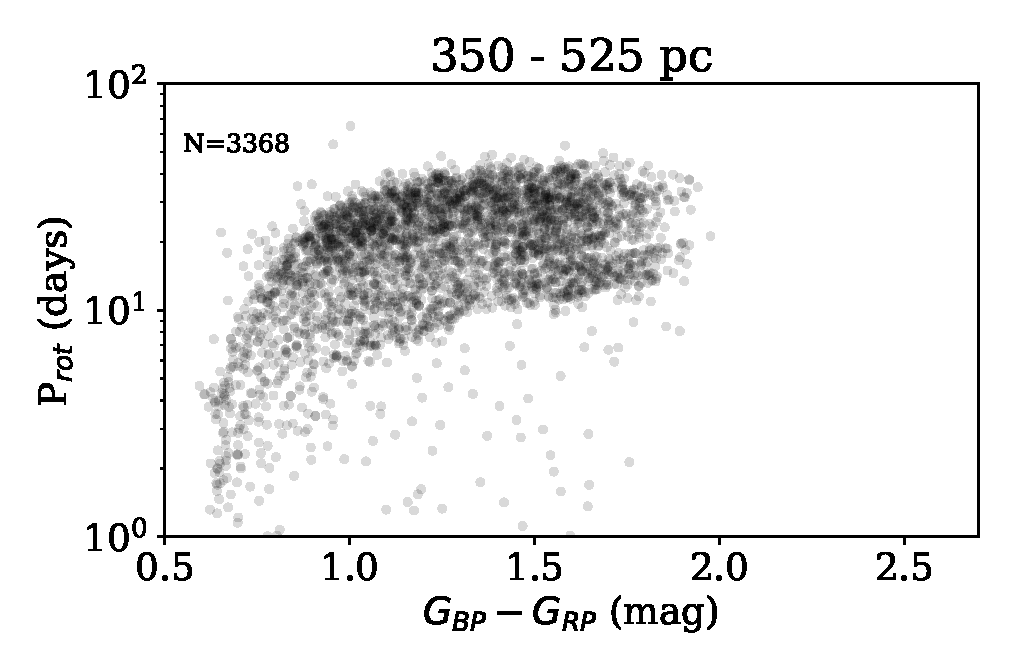
\includegraphics[width=3.5in]{../figures/rot_dist_350}
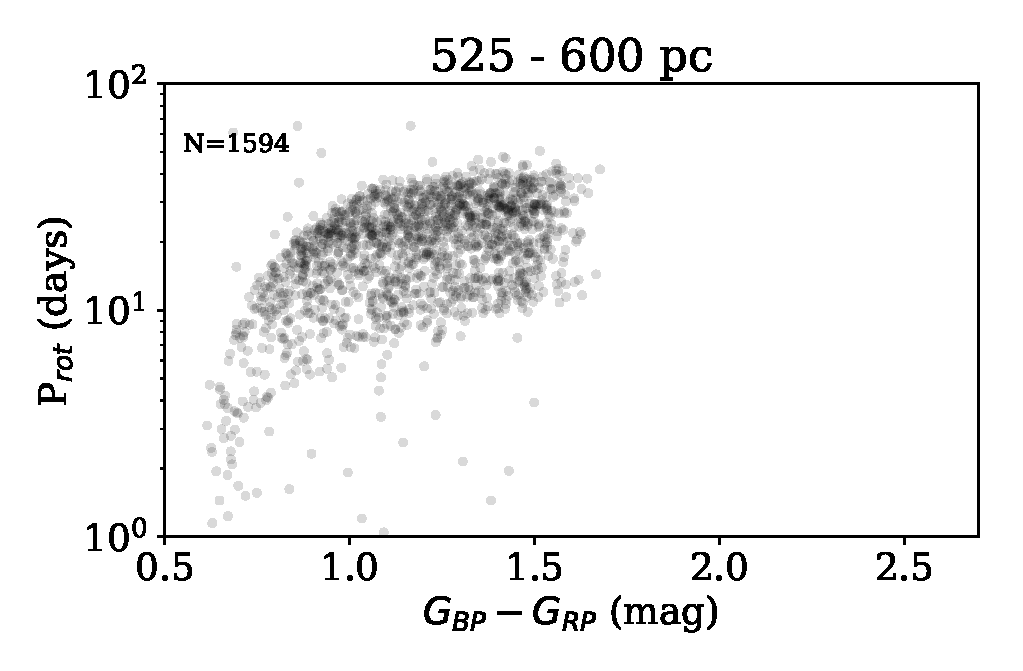
\includegraphics[width=3.5in]{../figures/rot_dist_525}
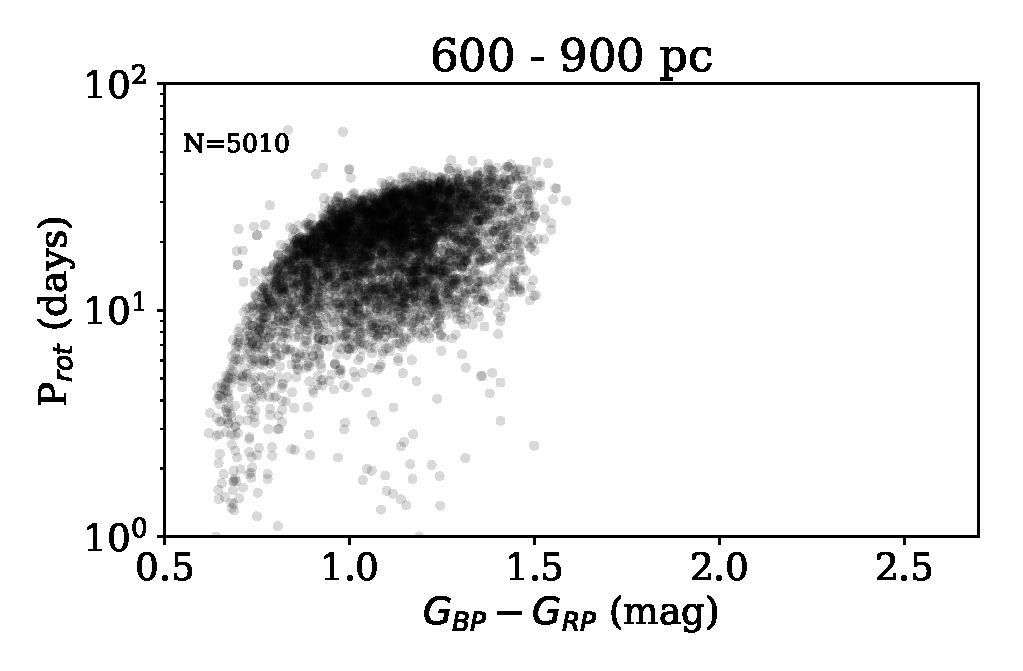
\includegraphics[width=3.5in]{../figures/rot_dist_600}
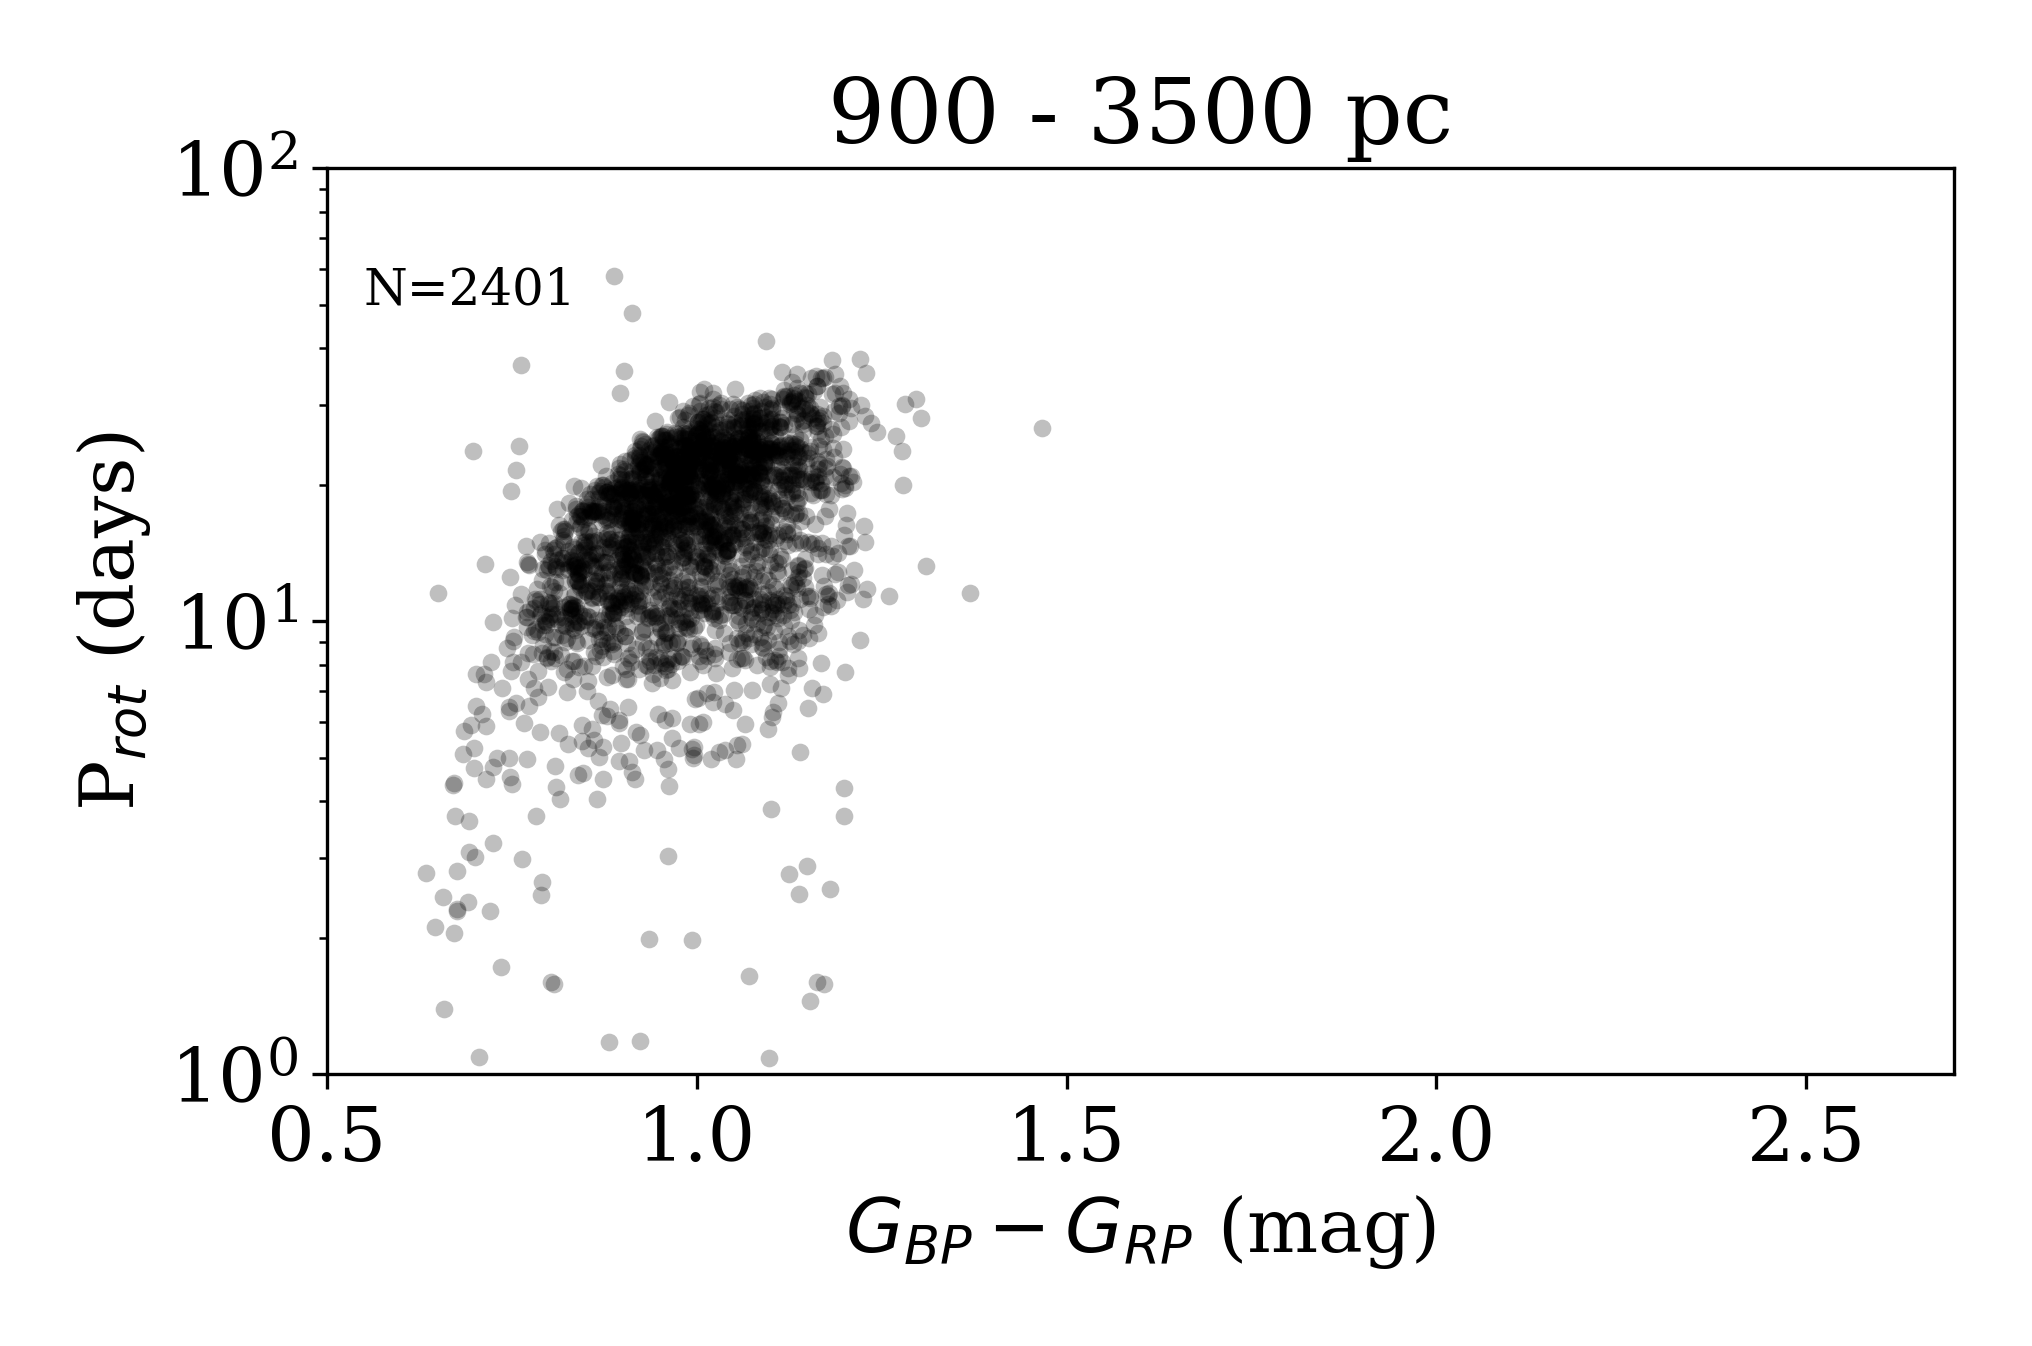
\includegraphics[width=3.5in]{../figures/rot_dist_900}
\caption{Color--period diagrams for our sample of likely main sequence stars, divided into bins of distance. Our nearest bin (within 350pc) is effectively the distance analyzed in \citet{davenport2017} using Gaia DR1, and clearly shows the rotation period bimodality for the entire sample. The brighter magnitude limit of the \Kepler sample results in redder (fainter) stars missing in our further distance bins. The rotation period bimodality can be seen in the 350-525 pc bin, but is not found in the bluer stars at further distances.
}
\label{fig:color_period}
\end{figure*}



%\begin{figure}[]
%\centering
%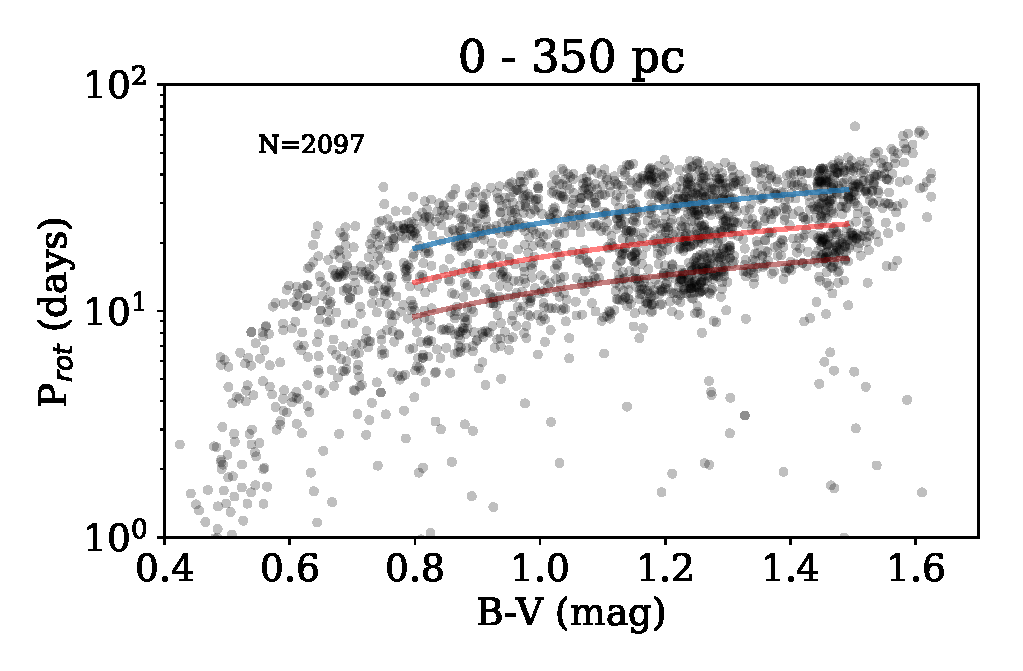
\includegraphics[width=3.5in]{../figures/B_V_rot}
%\caption{converted to B-V using Padova isochrone colors. 3 gyrochrones from \citet{meibom2009} with ages 300 Myr (dark red), 600 Myr (bright red), and 1.2 Gyr (blue) are shown.
%}
%%\label{fig:cmd}
%\end{figure}
%


\begin{figure}[]
\centering
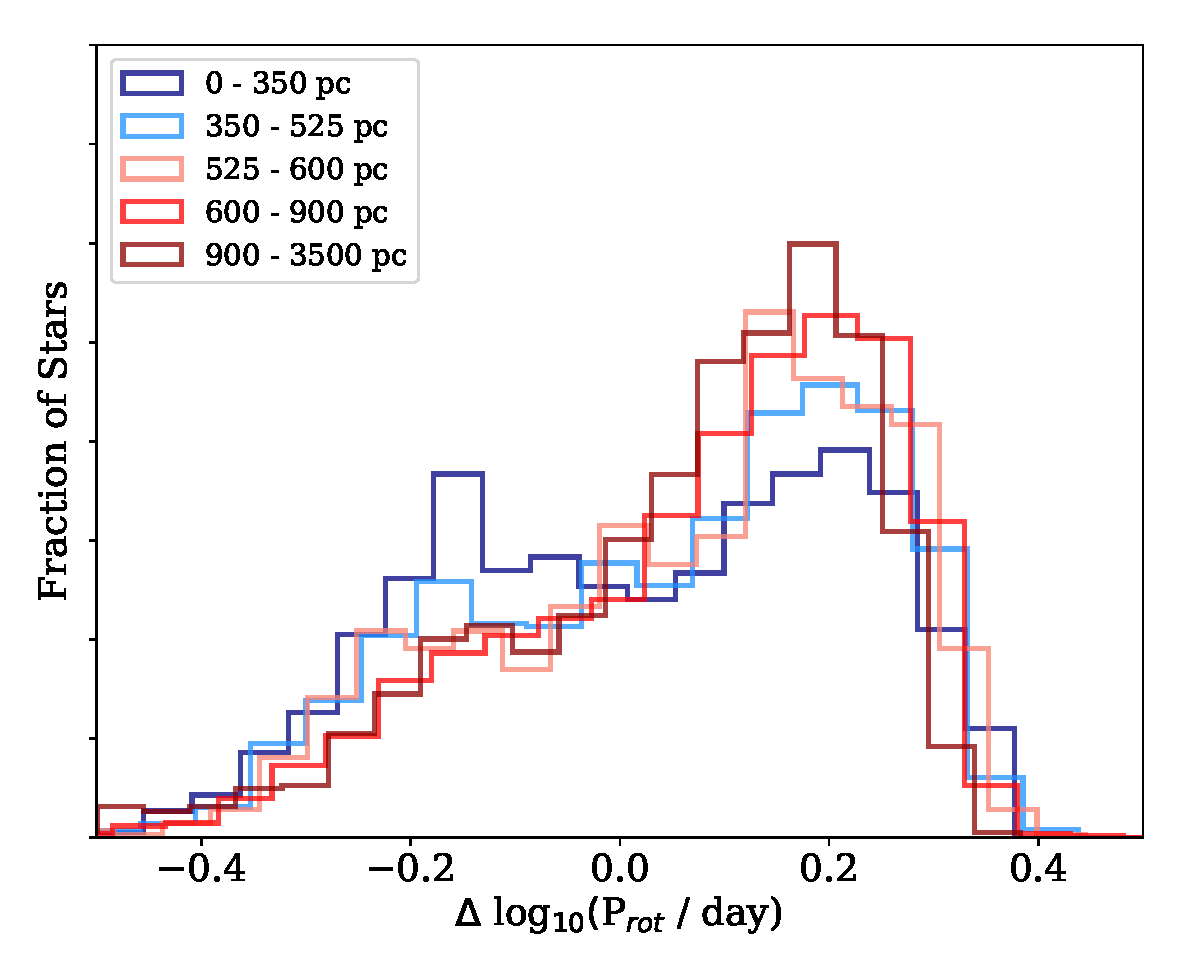
\includegraphics[width=3.5in]{../figures/delta_per}
\caption{Histograms of the log rotation periods after a 600 Myr gyrochrone was subtracted for stars in the same five distance bins shown in Figure \ref{fig:color_period}. The period bimodality for stars within 350 pc has two peaks similar to those found in \citet{davenport2017}, at -0.15 and +0.18 dex. The fast rotating peak (left side) declines sharply at further distances, however.
}
\label{fig:per_hist}
\end{figure}





\begin{figure*}[]
\centering
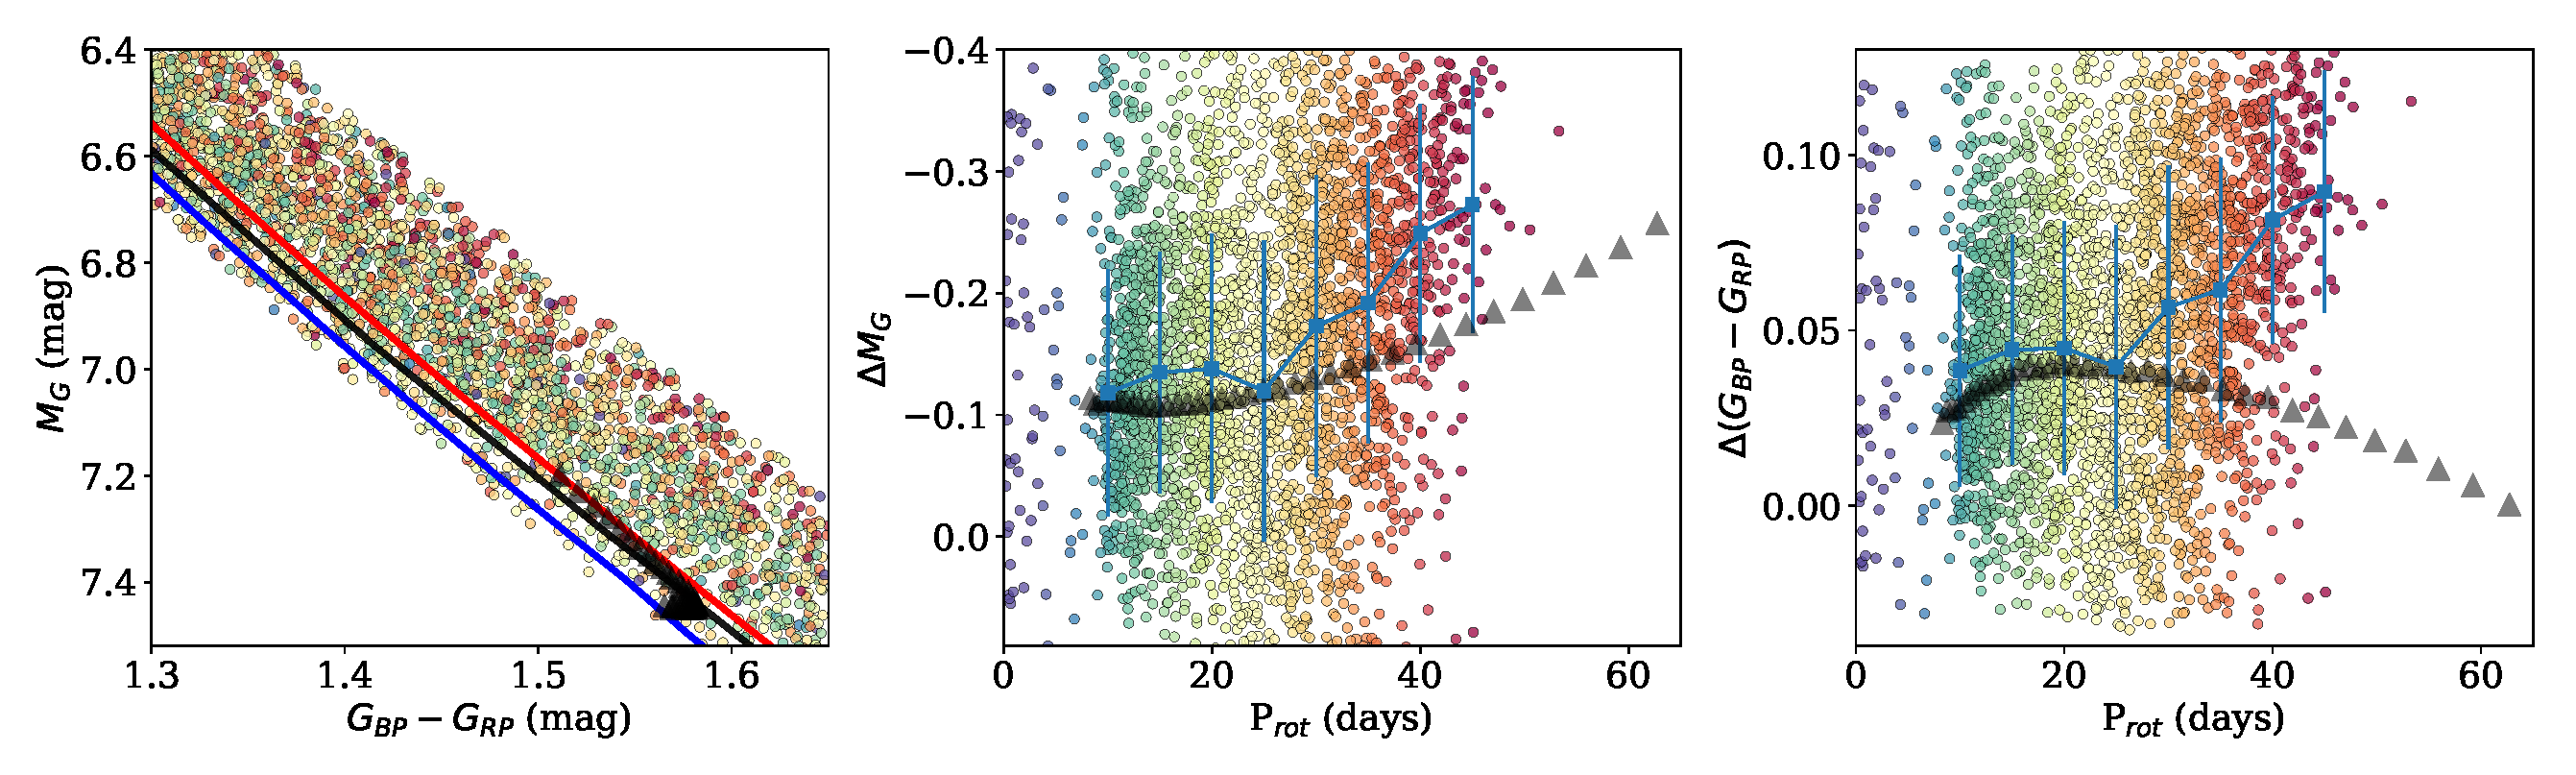
\includegraphics[width=6.5in]{../figures/cmd_zoom}
\caption{Left: Enlarged portion of the color--magnitude diagram from Figure \ref{fig:cmd} in a region centered near $\sim$0.75 M$_\odot$, with MIST isochrones at ages of $10^8$, $10^9$, and $10^10$ yr for comparison (blue, black, and red lines). Points are colored by their measured \Kepler rotation periods from \citet{mcquillan2014}. The main sequence shows significant scatter, as well as a gradient in rotation period. Right: Difference in $M_G$ from the $10^9$ yr MIST isochrone, shown as a function of their rotation periods (point color again indicates rotation period). Blue squares show an increase in the median $M_G$ offset in bins of increasing rotation period. Error bars shown are the standard deviation of $\Delta M_G$ in each bin.
}
\label{fig:cmd_zoom}
\end{figure*}




%\begin{figure}[]
%\centering
%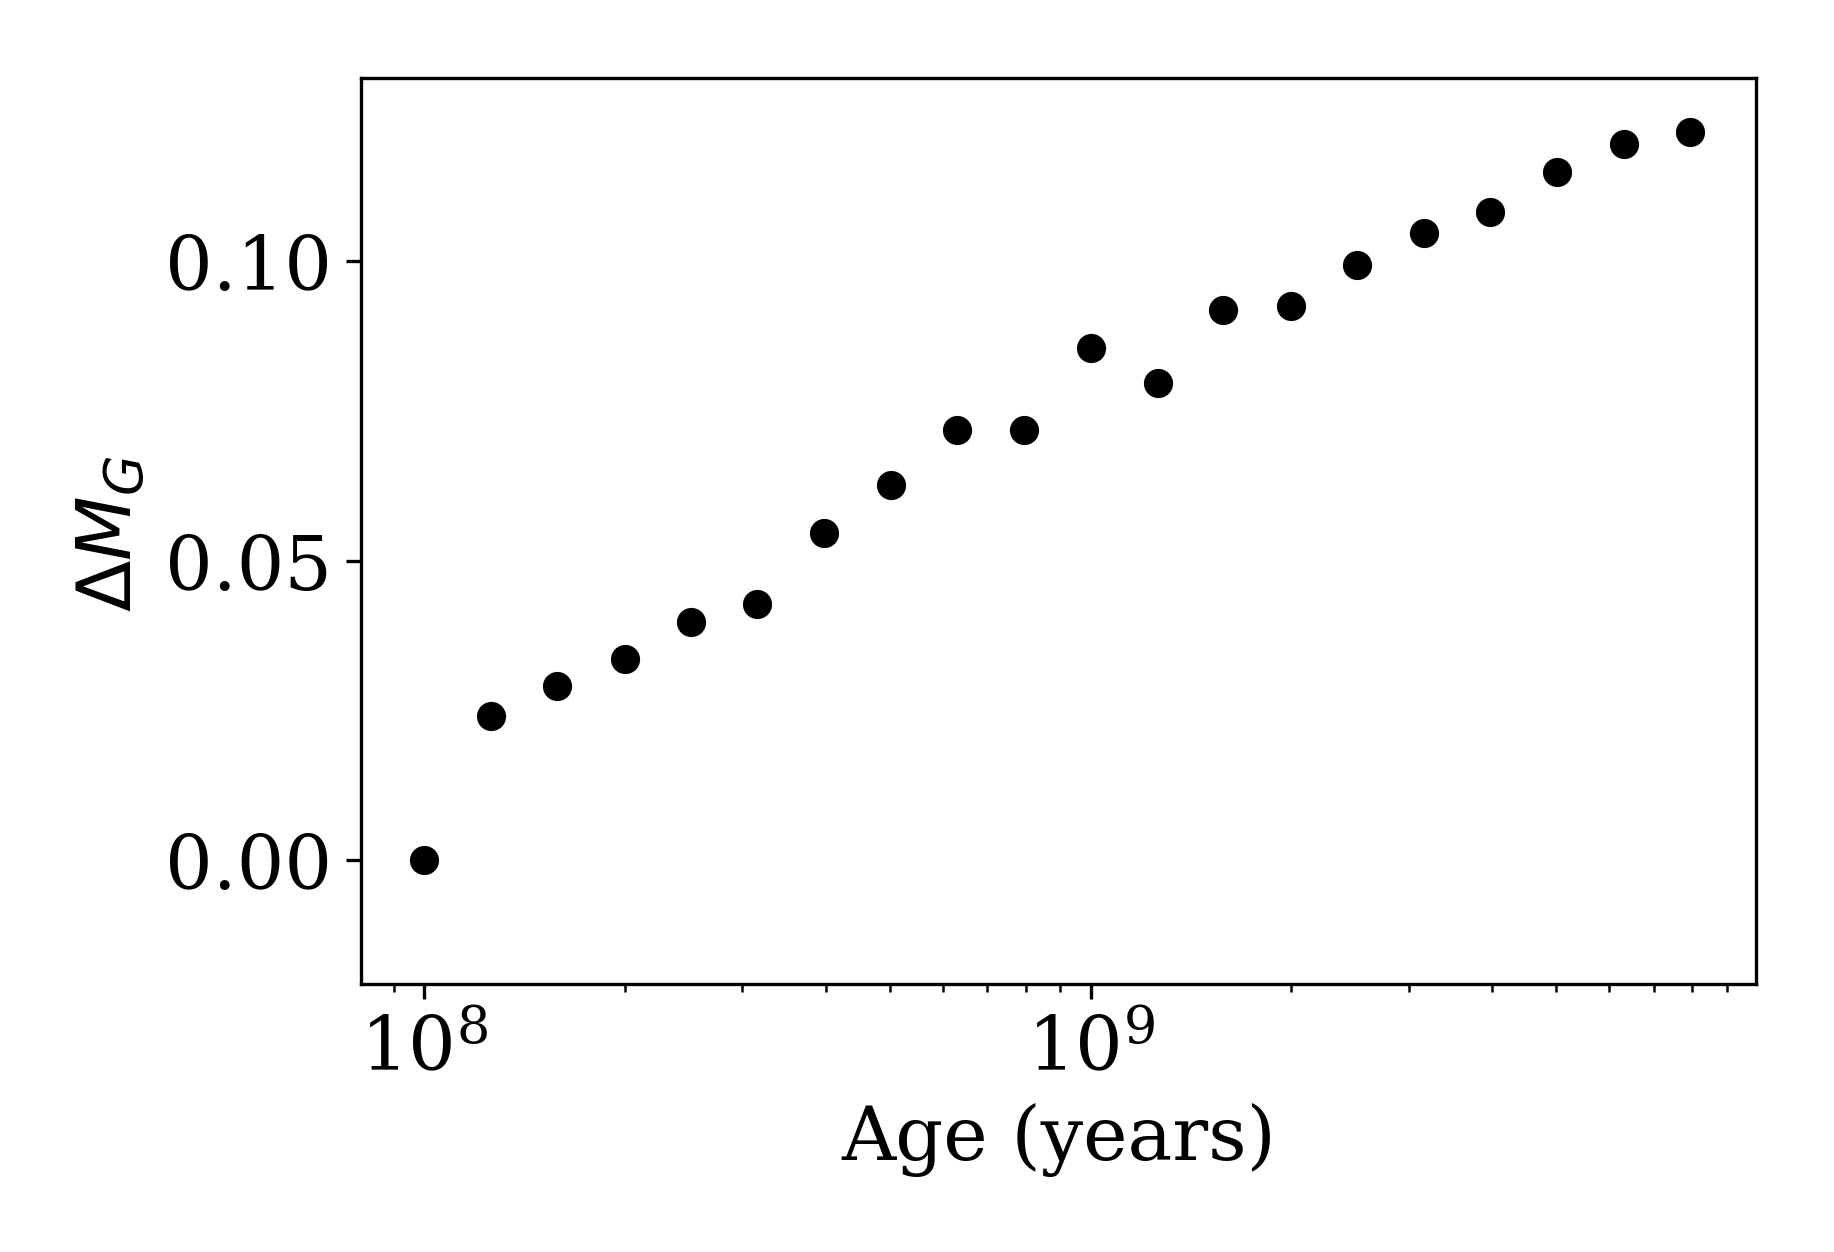
\includegraphics[width=3.5in]{../figures/iso_age}
%\caption{
%}
%%\label{fig:cmd}
%\end{figure}



%%%%%%%%%%%%%%%%%%%%%%
\section{Discussion}
%
%Using a combination of data from \Kepler and Gaia DR1, I have explored the rotation period distribution for 440 nearby main sequence stars. A bimodal rotation period distribution has been found in stars with temperatures ranging from 5000 K to 6500 K. This feature matches that found in cooler stars from \Kepler, but was only revealed thanks to the enhanced ability to distinguish dwarfs from subgiants using Gaia data. 
%A tenuous difference in the TGAS total proper motion for stars in the fast and slow rotating groups is found, which is in agreement with the findings for cool stars by \citet{mcquillan2013}.
%
%While a definitive explanation for this period bimodality has not been reached, the findings to date seem to favor stellar ages as the cause. In this scenario the star formation history for nearby stars would be dominated by two epochs of star formation, one short event centered at a few hundred Myr, and one long event centered at a few Gyr (slightly younger than the Sun). It is also worth noting that the space volume probed by the TGAS sample investigated here is very similar to that covered by the temperature-selected cool star sample in \citet{mcquillan2013}. The median parallax distance for stars in this work is 285 pc, while the median isochrone distance for the K and M dwarfs is $\sim$216 pc. This points to the period distribution being a localized age artifact. 
%Determining how localized this age distribution is, and if it can be confirmed for stars across the HR diagram including giants, is a key goal for future Gaia data releases.
%
%
%The period bimodality may yet be a manifestation of the ``Vaughan-Preston'' gap observed in chromospheric activity indicators from solar type stars. Such a feature has also been discussed for rotating stars by \citet{kado-fong2016}. Given that the mass range for the bimodality explored here and in \citet{mcquillan2014} covers stars with solar-type dynamos (those having a tachocline, late F through early M) such a model cannot be fully ruled out at this time. Though there have been many rotation studies for cool stars \citep[e.g.][]{irwin2011,newton2016,stelzer2016} too few rotation periods have been measured for stars across the ``fully convective boundary'' ($T_{eff}<3000$ K, spectral type $\sim$M4) to tell if the bimodal period feature continues to cooler temperatures, which would support the age distribution model. 
%If the bimodality is due to stars crossing a phase of rapid angular momentum evolution, we would expect to see it in stellar clusters at or near the critical age. The lack of this feature in the clusters observed to date could be due to no cluster being close enough to the critical age, which the gyrochrone in Figure \ref{fig:gyro} shows is near 600 Myr. Further studies of rotation periods for stars in intermediate age open clusters (e.g. the Hyades) may help solve this mystery \citep[e.g.][]{douglas2014}.
%
%Finally, this exploratory work has highlighted the utility of using astrometric data from Gaia combined with detailed light curve statistics from \Kepler to reveal hidden substructure in the properties of field stars. Looking forward to the astrometric precision of future Gaia data releases, this combination will be effective at separating dwarf stars from subgiants for nearly the entire \Kepler and K2 databases, and enable accurate age maps for field stars.



%%%%%%%%%%%%%%%%%
\acknowledgments

JRAD is supported by an NSF Astronomy and Astrophysics Postdoctoral Fellowship under award AST-1501418. 

This work made use of the \url{gaia-kepler.fun} crossmatch database, created by Megan Bedell.

This project was developed as part of the 2018 NYC Gaia Sprint, hosted by the Center for Computational Astrophysics at the Simons Foundation in New York City.


This work has made use of data from the European Space Agency (ESA) mission
{\it Gaia} (\url{https://www.cosmos.esa.int/gaia}), processed by the {\it Gaia}
Data Processing and Analysis Consortium (DPAC,
\url{https://www.cosmos.esa.int/web/gaia/dpac/consortium}). Funding for the DPAC
has been provided by national institutions, in particular the institutions
participating in the {\it Gaia} Multilateral Agreement.



\bibliography{/Users/davenpj3/Dropbox/references}

\end{document}
